\section{The laboratory notebook}
\subsection{The aim}
\begin{frame}[<+->]{Paper version}
\begin{textblock*}{10cm}(1cm,2cm) % {block width} (coords)
Laboratory notebook allow to:
\begin{itemize}
	\item Day-to-day recording each step in a process, experiments...
	\item Report on the progress, and scientific experimentations \newline
	from the idea to final conclusions
	\item Keep track of knowledge in a lab
	\item Useful drafting a patent
	\item Proof of anteriority
\end{itemize}
\end{textblock*}
\only<1>{
\begin{textblock*}{10cm}(1cm,3cm) % {block width} (coords)
  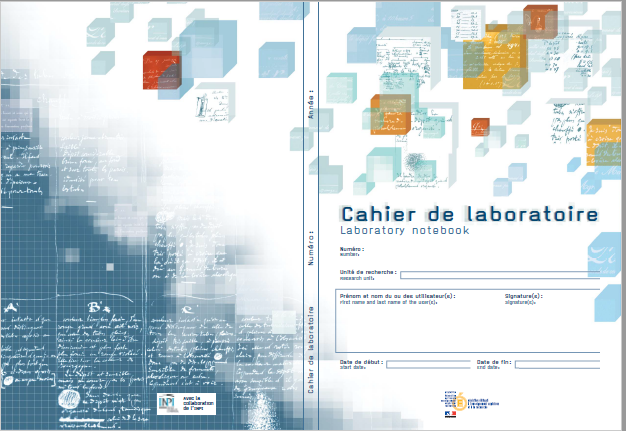
\includegraphics[width=7cm,height=5cm]{images/cahierlabo.png}
 \end{textblock*}
 \begin{textblock*}{10cm}(8cm,3cm) % {block width} (coords)
  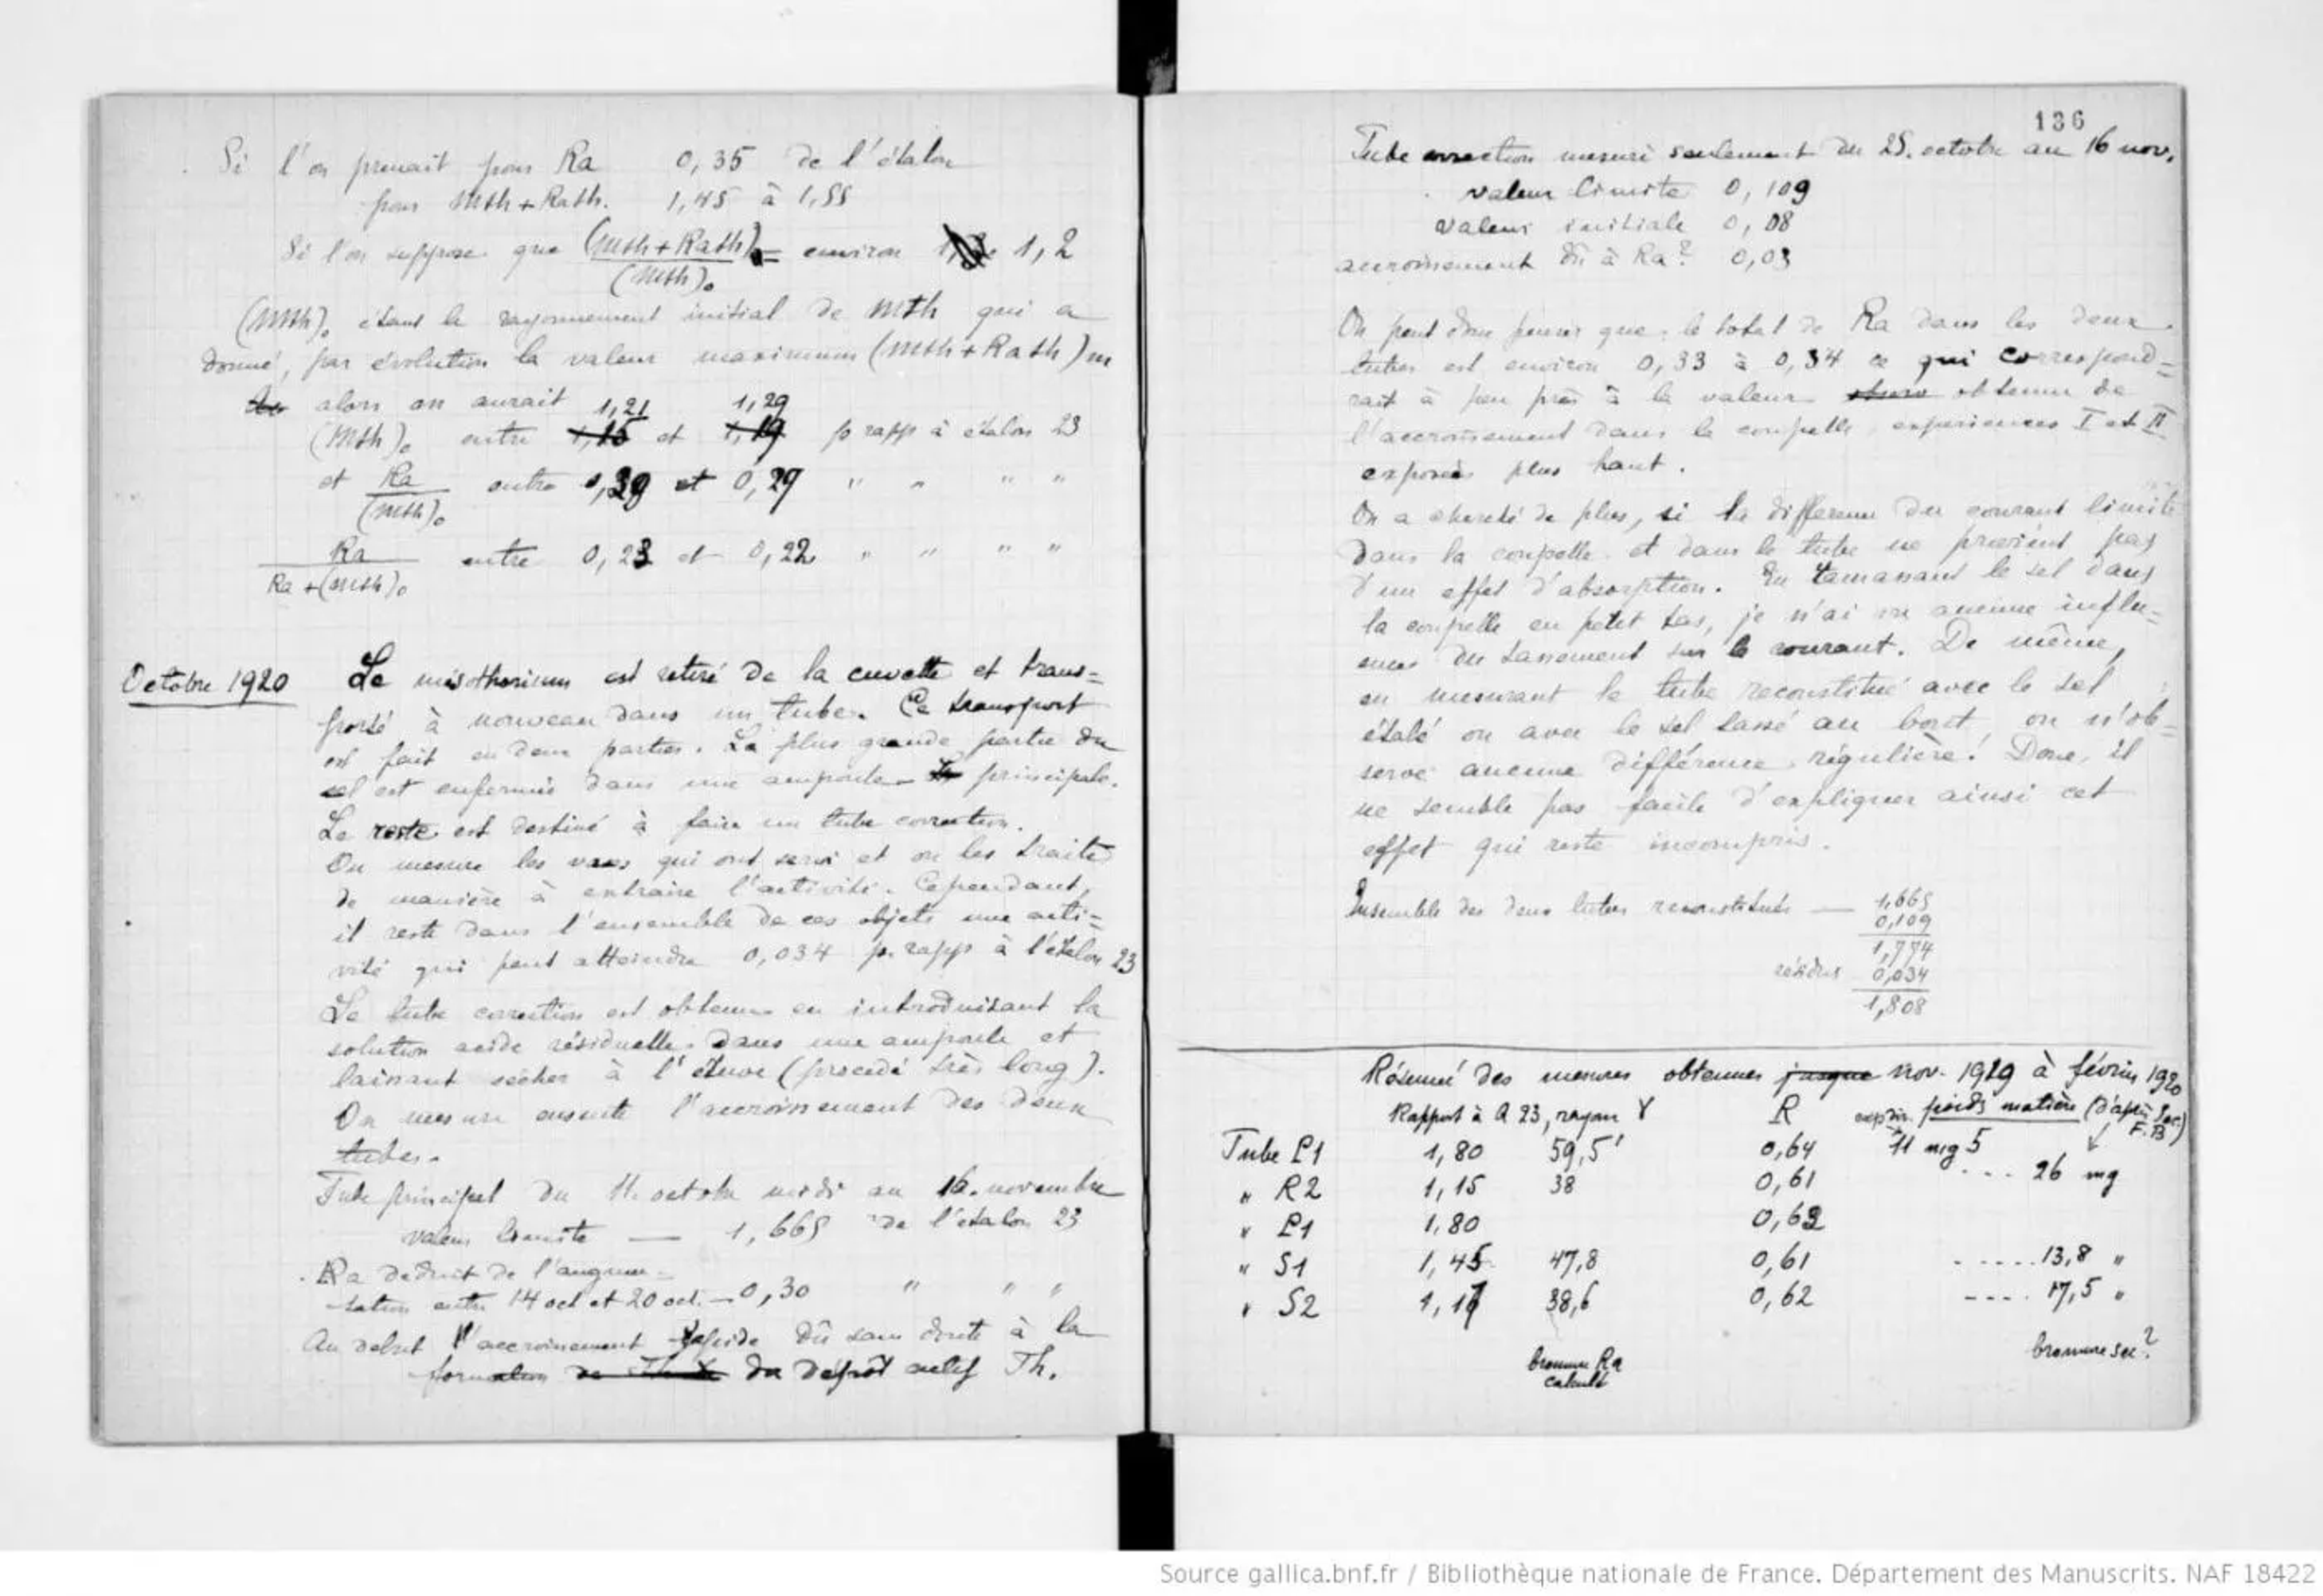
\includegraphics[width=7cm,height=5cm]{images/cahier2.pdf}
 \end{textblock*}}
\end{frame}

\begin{frame}[<+->]{Paper version}
\begin{columns}
\column{.5\textwidth}
This is a legal tool:
 \begin{itemize}
 \item Page numbered in each notebook
 \item Cover page with the owner of the results
 \item Each page contain a part to date, to sign for at least to people
 \end{itemize}
\column{.5\textwidth}
At each research level:
  \begin{itemize}
 \item Researchers
 \item Engineers
 \item Technicians
 \item Students...
 \end{itemize}
\end{columns}
\vspace{1cm}
\onslide<10>{\centering End what's happen for bioinformatic ?}
\end{frame}

\begin{frame}[<+->]{Electronic version}
\onslide<1->{Electronic Laboratory Notebooks (ELN)} \newline
\onslide<1->{Modern LN since 2009 (C.U.R.I.E. Network)}
\only<2>{
\begin{textblock*}{10cm}(9cm,2cm) % {block width} (coords)

\includegraphics[width=3cm,height=1cm]{images/elabftw-logo.png}
\end{textblock*}
\begin{textblock*}{10cm}(0.5cm,4cm) % {block width} (coords)
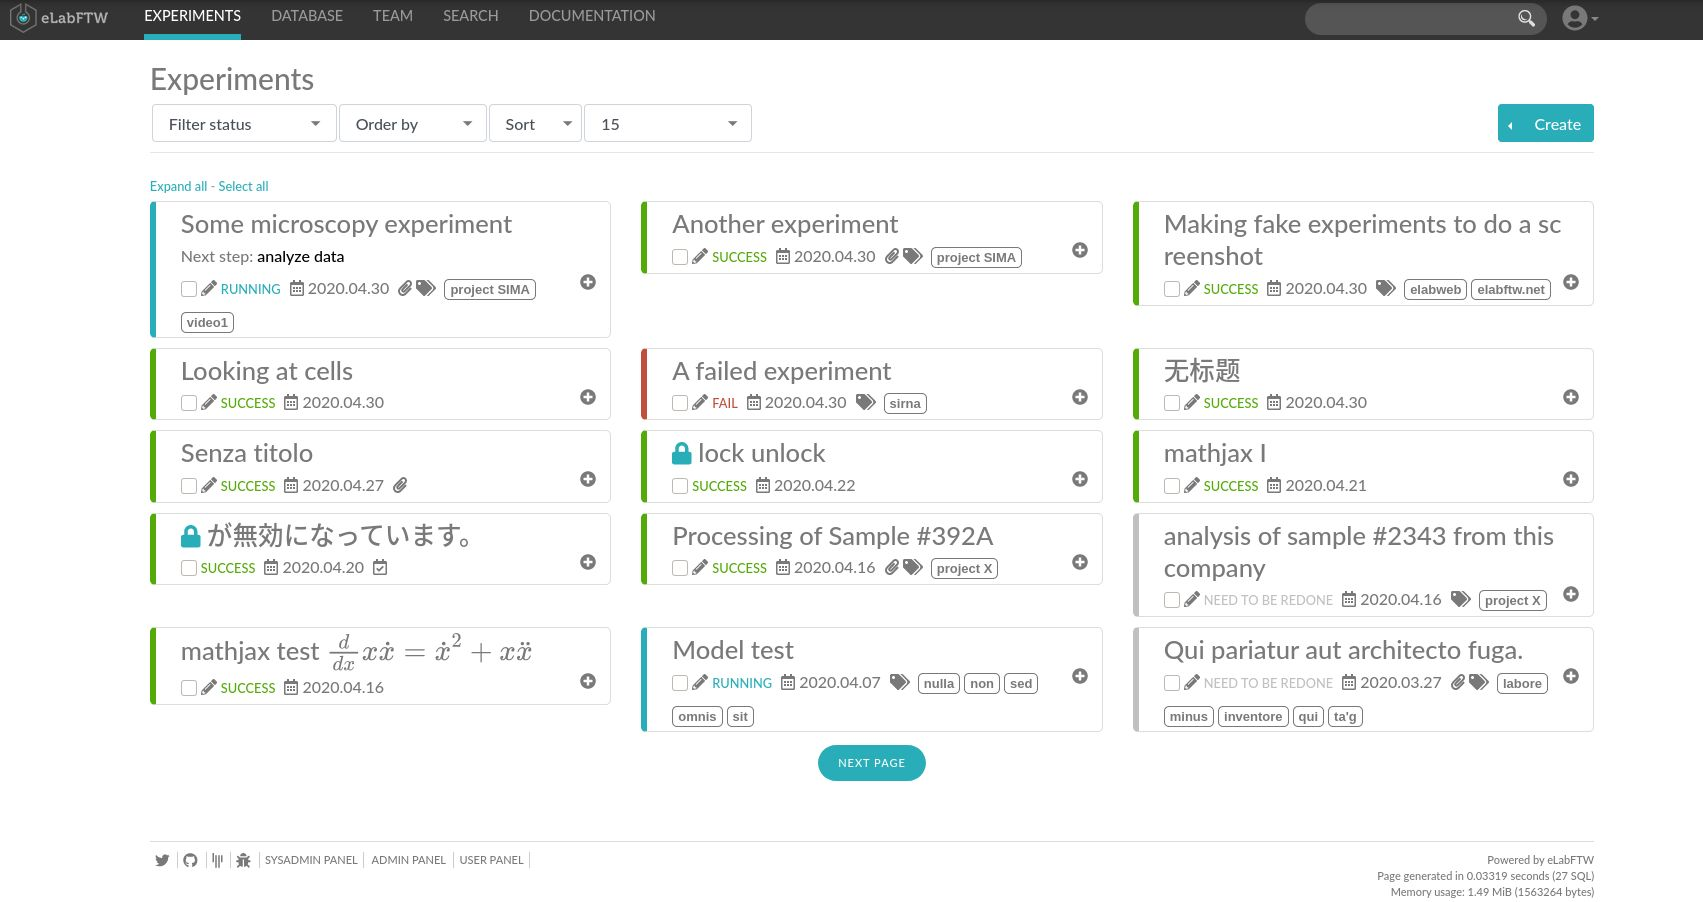
\includegraphics[width=7cm,height=4cm]{images/elabftw1.jpg}
\end{textblock*}
\begin{textblock*}{10cm}(8cm,4cm) % {block width} (coords)
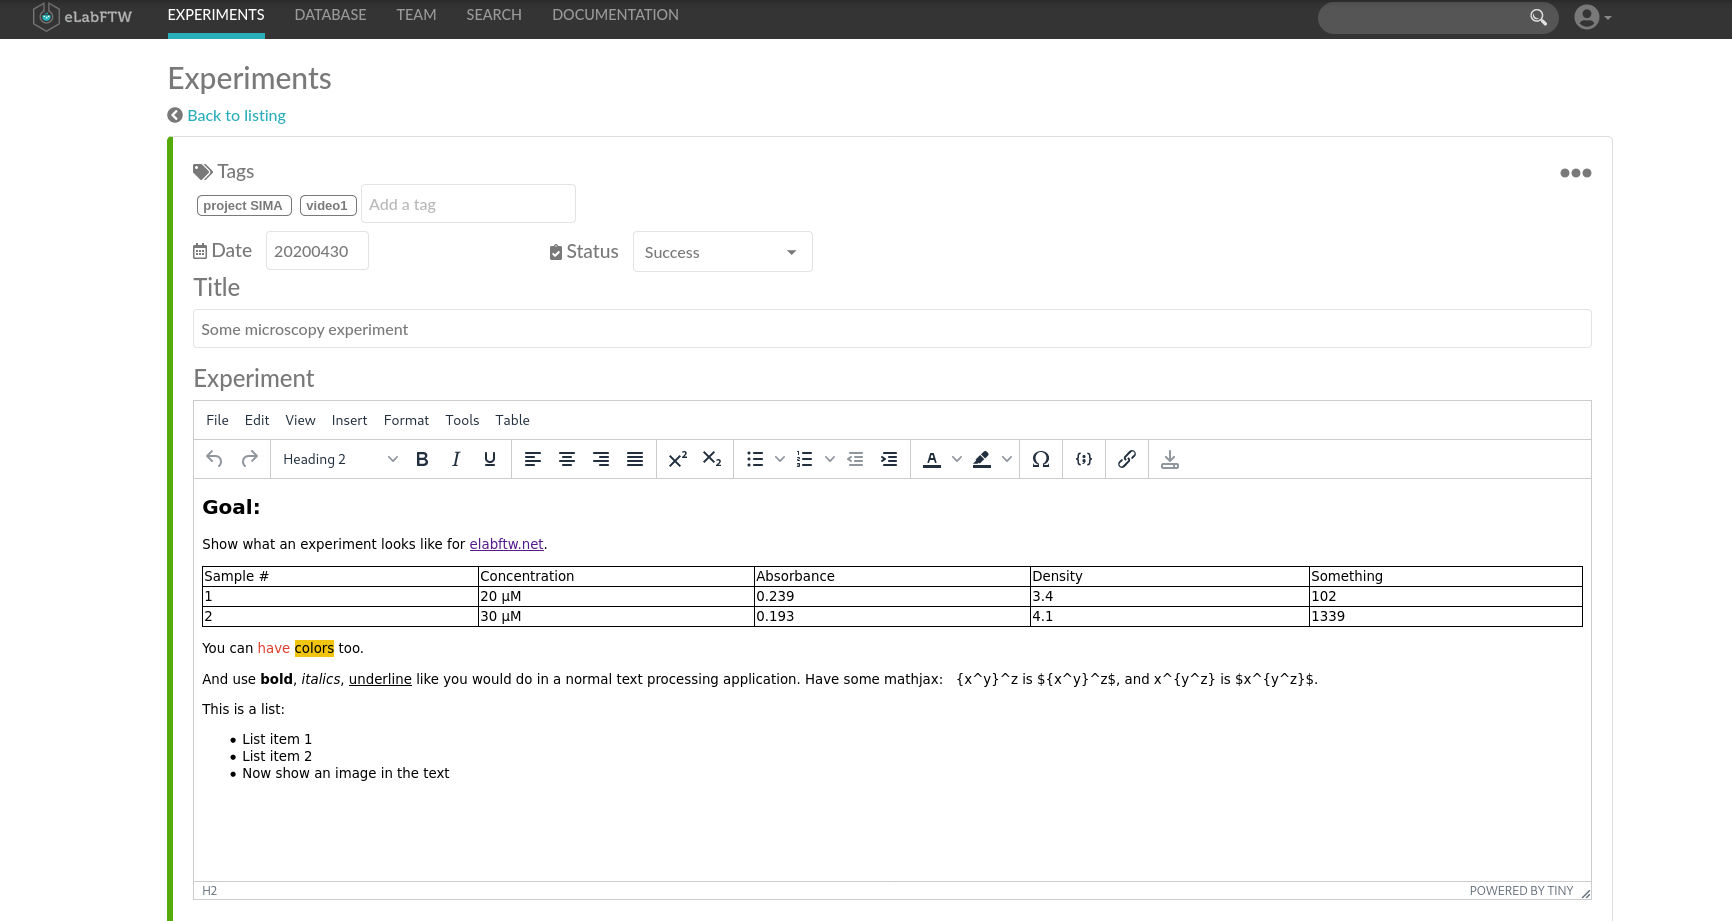
\includegraphics[width=7cm,height=4cm]{images/elabftw2.jpg}
\end{textblock*}}
\onslide<3->{
 \begin{itemize}
 	\item dematerialised
 	\item archivable
 	\item sharable
 	\item secure
 \end{itemize}}
\onslide<4->{
\centering But less and less adapted to recent evolutions of our work \\
\centering We need an electronic tool for individual traceability}
\end{frame}

\begin{frame}{Electronic version}
\only<1>{\centering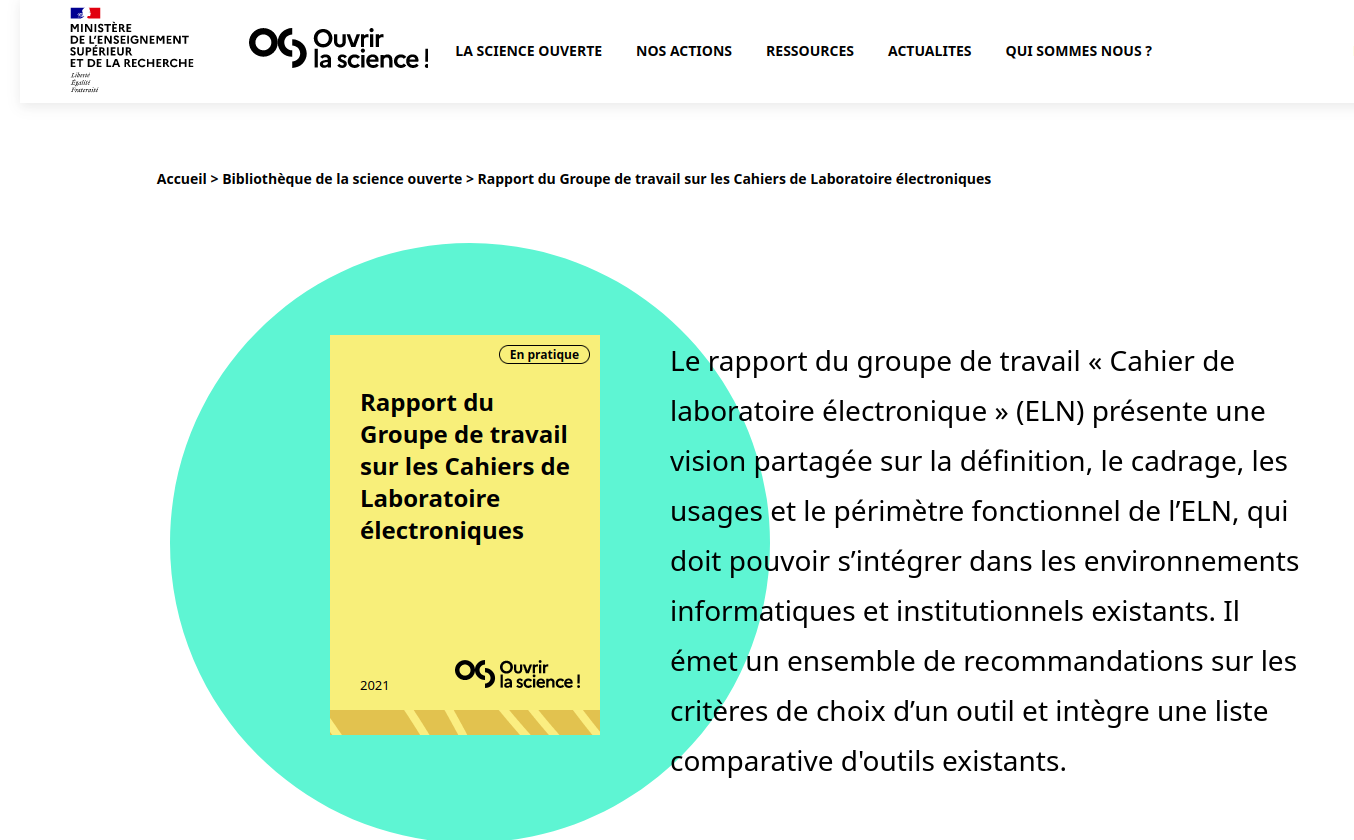
\includegraphics[width=10cm,height=7cm]{images/gt_eln.png}}
\only<2>{\centering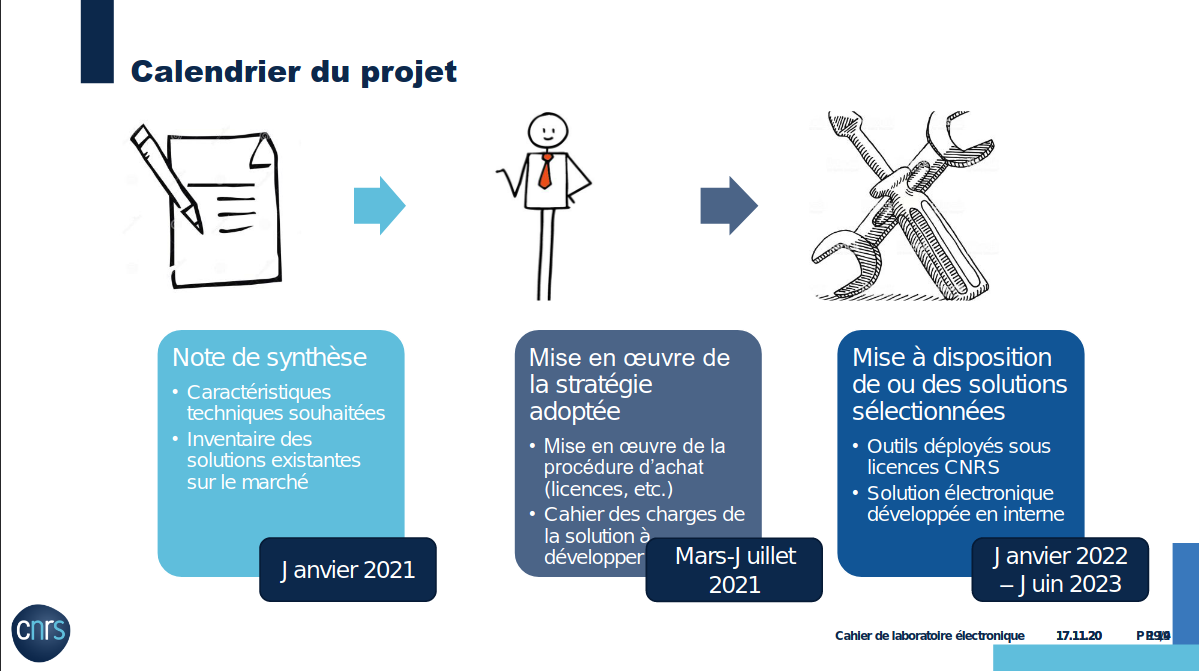
\includegraphics[width=10cm,height=7cm]{images/gt_eln_temp.png}}
\end{frame}

